\documentclass[11pt,letterpaper,twoside]{article}
\usepackage{fancyvrb,fancyhdr}
\usepackage{subfigure,tikz}
\usepackage{graphicx}
\usepackage{subfigure}
\usepackage{fancyhdr}
\usepackage{rotating}
\usepackage{multirow,multicol}
\usepackage{color}
\usepackage{float}
\usepackage{ifthen,verbatim}
\usepackage{amsmath,amsbsy,amssymb,bm}
\usepackage{mathrsfs}
\usepackage{longtable}
\usepackage{esvect}
\usepackage{listings}
\usepackage{enumerate}
\usepackage[parfill]{parskip}  
\usepackage{verbatim}
\usepackage[T1]{fontenc}
% Packages for algorithm environment
\usepackage{algorithmic}
\usepackage[ruled]{algorithm2e}
\usepackage{epstopdf}
\usepackage{bigstrut}

\usepackage{exercise}
\usepackage{flexisym}
\usepackage{arydshln}
\usepackage{enumerate}
\definecolor{shadecolor}{gray}{0.9}
\newcommand{\N}{\mathcal{N}}
\newcommand{\R}{\mathbb{R}}
\newcommand{\inv}{^{-1}}
\newcommand{\x}{\times}
\newcommand{\vu}{\vec{u}}
% \newcommand{\vv}{\vec{v}}
\newcommand{\vx}{\vec{x}}
\newcommand{\vb}{\vec{b}}
\newcommand{\vz}{\vec{z}}
\newcommand{\vw}{\vec{w}}
\newcommand{\ve}{\vec{e}}
\newcommand{\vr}{\vec{r}}
\newcommand{\vy}{\vec{y}}
\newcommand{\vq}{\vec{q}}
\newcommand{\va}{\vec{a}}
\newcommand{\vc}{\vec{c}}
\newcommand{\vd}{\vec{d}}
\newcommand{\vxk}{\vec{x}^{(k)}}
\newcommand{\vxko}{\vec{x}^{(k+1)}}
\newcommand{\alk}{\alpha^{(k)}}
\newcommand{\pk}{\vec{p}^{(k)}}
\newcommand{\rk}{\vec{r}^{(k)}}
\newcommand{\rko}{\vec{r}^{(k+1)}}
\newcommand{\vf}{\vec{f}}
\newcommand{\vT}{\vec{T}}
\newcommand{\la}{\lambda}
\newcommand{\then}{\rightarrow}
\newcommand{\bmat}[1]{\begin{bmatrix}#1\end{bmatrix}}
\usepackage{enumitem,parallel}	% allows for paragraph indentation within enumerate environment

\newcommand{\overto}[1]{\overset{#1}{\longrightarrow}}
\newcommand{\dxtwo}[1]{\frac{d^2#1}{dx^2}}

\newcommand{\half}{\frac{1}{2}}
\newcommand{\twith}{\text{ with }}
\newcommand{\tand}{\text{ and }}
\newcommand{\tfor}{\text{ for }}

\newcommand{\pars}[1]{\ensuremath{\left(#1\right)}}
\newcommand{\brks}[1]{\ensuremath{\left[#1\right]}}
\newcommand{\brcs}[1]{\ensuremath{\left\{#1\right\}}}
\newcommand{\angs}[2][]{\ensuremath{{\vphantom{\left\langle#2\right\rangle}}_{#1\!}\left\langle#2\right\rangle}}
\newcommand{\norm}[1]{\ensuremath{\left\|#1\right\|}}
\newcommand{\abs}[1]{\ensuremath{\left|#1\right|}}

\newcommand{\parscond}[2]{\ensuremath{\left(#1\vphantom{#2}\ \right|\left.\vphantom{#1}#2\right)}}
\newcommand{\brkscond}[2]{\ensuremath{\left[#1\vphantom{#2}\ \right|\left.\vphantom{#1}#2\right]}}
\newcommand{\brcscond}[2]{\ensuremath{\left\{#1\vphantom{#2}\ \right|\left.\vphantom{#1}#2\right\}}}
\newcommand{\angscond}[2]{\ensuremath{\left\langle#1\vphantom{#2}\ \right|\left.\vphantom{#1}#2\right\rangle}}


\newcommand\overmat[2]{%
  \makebox[0pt][l]{$\smash{\overbrace{\phantom{%
    \begin{matrix}#2\end{matrix}}}^{\text{$#1$}}}$}#2}
\oddsidemargin 0in \evensidemargin 0in
\topmargin -0.5in \headheight 0.25in \headsep 0.25in
\textwidth 6.5in \textheight 9in %\marginparsep 0pt \marginparwidth 0pt
\parskip 0ex \parindent 0ex \footskip 20pt


\def\ni{\noindent }
\allowdisplaybreaks[4]
\let \ds \displaystyle

% Environment for problem solution and rubric
\newboolean{showsolutions}
\newboolean{showrubric}
% Set showsolutions and showrubric to 'true' or 'false'
\setboolean{showsolutions}{false}
\setboolean{showrubric}{true}
\newenvironment{code}%
   {\color{gray!100}\verbatim}%
   {\endverbatim}
\newenvironment{solution}
{
  \ifthenelse{\boolean{showsolutions}}
  {\color{blue}\par\smallskip\underline{\textbf{Solution}}\par\medskip}
  {\expandafter\comment}
}
{
  \ifthenelse{\boolean{showsolutions}}
  {}
  {\expandafter\endcomment}
}

\newenvironment{rubric}
{
  \ifthenelse{\boolean{showrubric}}
  {\color{red}\par\medskip\underline{\textbf{Suggested Rubric}}\par\medskip\begin{itemize}}
  {\expandafter\comment}
}
{
  \ifthenelse{\boolean{showrubric}}
  {\end{itemize}}
  {\expandafter\endcomment}
}


% Used for drawing a pretty circle
%\drawsector[]{text radius}{width}{start angle}{delta angle}{text}
\newcommand{\drawsector}[6][]{
    \draw[#1] (#4:{#2-.5*#3}) arc [start angle = #4, delta angle=-#5, radius={#2-.5*#3}]--++({#4-#5}:#3) arc [start angle = {#4- #5}, delta angle=#5, radius={#2+.5*#3}] --cycle;
\draw[decorate,decoration={raise=-3pt, text along path, text=#6, text align={align=center}}] (#4:#2) arc(#4:(#4-#5):#2);
}
\usetikzlibrary{decorations.text}
\usepackage[hidelinks]{hyperref}
\hypersetup{
    colorlinks,
    linkcolor=blue,
    citecolor=blue,
    urlcolor=blue
    }
\usepackage{totcount}
\newtotcounter{max_points}
\setcounter{max_points}{0}
\newcommand\printpoints{Total number of points: \total{max_points}.}
\newcommand\setpoints[1]{\addtocounter{max_points}{#1}(#1 points)}
\newcommand\aug{\fboxsep=-\fboxrule\!\!\!\fbox{\strut}\!\!\!}


%\addtolength{\topmargin}{-.5in}
\begin{document} \pagestyle{empty}
\begin{minipage}[t]{0.6\linewidth}
  {\small\it STAT 494\\
     L. Lyman \\
     Spring 2023}
\end{minipage}
\hfill
%\bigskip\bigskip

\smallskip

\begin{center}
\textbf{Assignment 1
\ifthenelse{\boolean{showsolutions}}
{\color{blue}{-- Solution}}{}
}

\medskip
Due: \textbf{Wednesday, February 15}, by 11:59 pm CST\\
Submitted in class, or emailed to the instructor \\
%No late assignments accepted\\

\medskip


\end{center}
\medskip

\begin{quote}
We demand rigidly defined areas of doubt and uncertainty! --- \emph{The Hitchhiker’s Guide to the Galaxy}, \textsc{Douglas Adams}
\end{quote}

\bigskip

\textbf{Instructions (Please read carefully before beginning)}

%\medskip
%%%MMMM Please use bullet points for the instructions
\smallskip
(i) You may submit your assignment in class or via email to \href{mailto:llyman@macalester.edu}{llyman@macalester.edu}.~(ii) The default programming language for this course is Python with Jupyter Notebooks. However, you are free to use the language of your choice (MATLAB, C\texttt{++}, etc.).~(iii) Export your answers (plots, numerical values, etc.), along with all code used to generate those answers, as a PDF. (iv) Use best coding practices when possible.~Extract repeated code with functions, use descriptive variable names, and add informative comments. (v) You are \textbf{encouraged to work with others}, but each person is responsible for submitting an individual writeup. (vi) You are required to do:
\begin{itemize}

\item Exercise 1
\item \textbf{\textsc{Either}} Exercise 2 \textsc{or} 3.
\end{itemize}

If you complete all exercises, you earn the highly-coveted title of \textbf{UQ Master}.

%\vspace*{-6pt}
\ni\rule{\linewidth}{1pt}
\medskip

\begin{enumerate}
\item (50 pts) \textbf{Nagel-Schreckenberg traffic modeling.} 
\smallskip

Recall that our traffic flow model has the following:

\smallskip
\begin{itemize}
\item A single lane
\item $M$ chunks of road, labeled $0, \ldots, M - 1$ (with $M > 1$)
\item $N$ total vehicles ($N \le M$)
\item Discrete time steps $t_0, t_1, \ldots$ of identical length
\end{itemize}
\medskip
We can picture the road via Figure \ref{NS-mod}.%\vspace{-10pt}
\begin{figure}[H]\label{NS-mod}  
\begin{center}
\scalebox{0.8}{
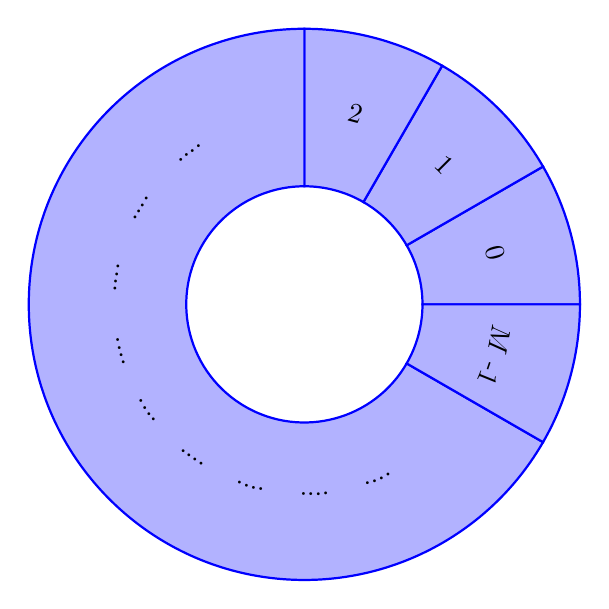
\begin{tikzpicture}
\drawsector[draw=blue,thick,fill=blue!30]{2.5}{2}{30}{30}{0}
\drawsector[draw=blue,thick,fill=blue!30]{2.5}{2}{60}{30}{1}
\drawsector[draw=blue,thick,fill=blue!30]{2.5}{2}{90}{30}{2}
\drawsector[draw=blue,thick,fill=blue!30]{2.5}{2}{330}{240}{....\ \ \ \ ....\ \ \ \ ....\ \ \ \ ....\ \ \ \ ....\ \ \ \ .... \ \ \ \ .... \ \ \ \ .... \ \ \ \ ....}
\drawsector[draw=blue,thick,fill=blue!30]{2.5}{2}{0}{30}{$M$ -1}
\end{tikzpicture}}
\end{center}
\vspace{-8pt}
\caption{A circular, one-way, single lane road with $M$ spots, labeled $0, \ldots, M - 1$.}
\end{figure}
 Further, we assume the following.
\smallskip
\begin{itemize}
\item Each vehicle occupies exactly one chunk at a given time step $t$ 
\item A car with velocity $v \ge 0$ moves $v$ spots forward in one time step
\item There is some speed limit $v_{\text{max}} > 0$
\end{itemize}

\medskip

\emph{Possible} pseudocode for the whole procedure could look like the following (Algorithm \ref{one-step}) for a \emph{single} time step. For indexing convenience, it is likely a good idea to label your cars such that car $i+1$ is in front of car $i$ for all $i \in \{0, \ldots, N-2\}$. 
\medskip

\setlength{\algomargin}{1em}
\centerline{
\begin{algorithm}[H]\label{one-step}
  \caption{\textbf{Nagel-Schreckenberg}}
  \textbf{input}  \begin{itemize} \item $M$, $N$, fixed probability 0 < $p$ < 1
\end{itemize} 
 \textbf{input (or initialize)}
 \begin{itemize}
 \item $\bm{x}$ \tcp{$N \times 1$ vector of car positions}
 \item $\bm{v}$  \tcp{$N \times 1$ vector of car velocities}
 \item $\bm{d}$  \tcp{$N \times 1$ vector of distances between cars, where $d_i = |x_{i+1\text{(mod}\thinspace N)} - x_i|$}
 \quad \tcp{ for $i = 0, \ldots, N -1$ }
 \end{itemize}
  \vspace{-5pt} \hrulefill \\ 
 \For{$i = 1, \ldots, N$}{
$(x_i, v_i) \gets \textbf{NS-update}(x_i, v_i, d_i, p)$
}
\textbf{update} $\bm{d}$ based on new $\bm{x}, \bm{v}$ \\
 \indent \Return $(\bm{x}, \bm{d}, \bm{v})$
    \end{algorithm}
}
\medskip
The following helper routine (Algorithm \ref{ns-update}) updates the $i$th car. 
If you prefer, Algorithm \ref{ns-update} could of course be modified to update all of the cars at once  by taking in vectors $\bm{x}, \bm{v}, \bm{d}$ of positions, velocities, and distances.

\medskip

\setlength{\algomargin}{1em}
\centerline{
\begin{algorithm}[H]\label{ns-update}
  \caption{\textbf{NS-update}}
  \textbf{input}  \begin{itemize} \item The position $x \in \{0, \ldots, M-1\}$ and velocity $v$ of the vehicle
  \item The distance $d$ between this vehicle and the car immediately in front of it
  \item Probability $0 < p < 1$ of randomly slowing down \end{itemize} 
 \vspace{-5pt} \hrulefill \\ 
  \tcp{Drivers are eager to move forward, so you speed up by 1 unit if you can. If you're already speeding, you (begrudgingly) slow down to the speed limit}
 \begin{itemize}
 \item \textbf{set} $v \gets \min(v + 1, v_{\text{max}})$ \hfill \textcolor{blue}{(1)}
 \end{itemize}
\tcp{You're worried about what would happen if the car in front of you suddenly stopped. If you'll crash into the car in front within one time step (i.e. if $v \ge d$), then slow down by 1 unit. Otherwise, continue at your current speed}
 \begin{itemize}
 \item \textbf{set} $v \gets \min(d-1, v)$ \hfill \textcolor{blue}{(2)}
 \end{itemize}
 \tcp{This car is a metal death trap! With probability $p$, slow down by 1 unit (if you're not already stopped)}
  \begin{itemize}
 \item With probability $p$, \textbf{set} $v \gets \max(0, v-1)$ \hfill \textcolor{blue}{(3)}
 \end{itemize}
  \tcp{Based on your current speed, update the position}
  \begin{itemize}
 \item \textbf{set} $x \gets x + v  \mod M$ \hfill \textcolor{blue}{(4)}
 \end{itemize}
 \indent \Return $x$, $v$
    \end{algorithm}
}
\smallskip


\medskip
%As was pointed out in class, steps \textcolor{blue}{(1) - (3)} happen \emph{instantaneously}. That is, we assume a driver does the mental calculations for these velocity updates and then perfectly transitions to the new speed --- all in one time step. 

\smallskip




\medskip 
\begin{enumerate}
\item (12 pts) Create a Monte Carlo simulation of the Nagel-Schreckenberg traffic model. Let the number of spaces $M = 1,000$ and the number of cars $N = 50$. Take $v_{\max} = 35$ and $p = \frac{1}{3}.$ Initialize your simulation via the following.
\begin{itemize}
\item The cars have initial positions $x_i$ determined by sampling $N$ values from $\{0, \ldots, M - 1\}$ uniformly without replacement.
\item The $N$ cars have initial velocity $v_i = 0$. 
\item There is a "burn-in" period of 2,500 time steps. That is, let your simulation run for 2,500 time steps before ``starting the clock" to produce your figure for (b). 

\textbf{Note.} This terminology is \textbf{different} than what I described in class, in which the "burn-in" period was the time for which the simulation is run.
\end{itemize}
\medskip
\item (13 pts) Make a flow trace image analogous to Figure \ref{NS} for 1,000 time steps after the burn-in period. You should get something quite similar. Note that you might prefer to make $\bm{x}, \bm{v}, \bm{d}$ into matrices to keep track of your data per time step.
%\vspace{-10pt}
\begin{figure}[H]
\centerline{\includegraphics[scale=.7]{NSFig1}}
%\vspace{-10pt}
\caption{Flow trace image for NS traffic modeling.}\label{NS}
\end{figure}
\vspace{-10pt}
The dark bands represent the traffic jams.
\medskip

\item (2 pts) Since the road is one-way, any update formulas must preserve that all $v_i \ge 0$. Add a line in your code to verify this is the case. 
\medskip
\item (5 pts) Ben initiated an important discussion in class about whether certain velocity-updating steps should be permuted. That is, even if we imagine the velocity-updating steps occurring \emph{simultaneously}, there will ultimately be an order of execution in the code itself. Does the order of these steps matter? Try rearranging \textcolor{blue}{(1) - (3)} from Algorithm \ref{ns-update} in your code and state your observations. 
\medskip
\item (8 pts) I claimed in class that the slowing with probability $p$ in step  \textcolor{blue}{(3)}  is what \emph{causes} the jams to appear. Let's verify that in our simulation. Take out step (c) and run your model for some time. Do you observe any jams? 
\medskip
\item (10 pts) Sarah pointed out that for step \textcolor{blue}{(2)}, we might not crash into the car in front of us even if $v \ge d$, because the car ahead is also traveling forward by some velocity $v \ge 0.$ That is, we might be \emph{too} cautious by worrying about whether the car ahead will randomly stop. (How likely is that, anyway?) Instead, take out step \textcolor{blue}{(2)}. When re-computing $\bm{d}$ (e.g. after the \texttt{for} loop in Alg. \ref{one-step}), only force a car to slow down if it is actually going to collide with someone. What effect, if any, does this have on the traffic jams?

\medskip
\item \textbf{Bonus}. (Title of Ultimate UQ Star) Animate your graphic in time. Include your code, save your animation (e.g., as a GIF), and include a link to the animation in your submission. 
\end{enumerate}
\bigskip 
%%%%%%%%%%%%%%% Problem 1 %%%%%%%%%%%%%%%%%%%%

\item (50 pts) \textbf{Cutie $\pi$.}
\smallskip

Estimate $\pi$ by computing a Monte Carlo integral. If you didn't take notes in class that day, get them from a friend or ask me for them.
\medskip

This one is a classic problem for getting accustomed to integrating with Monte Carlo. You can likely find the answer on any data science blog online, but \textbf{try} to do this on your own. It is a good reality-check for whether you are internalizing the relevant concepts. 

\bigskip

\item (50 pts) \textbf{Orthogonal polynomials and Gaussian quadrature.}

\textbf{Note.} You might need to wait until after Monday's lecture (on 2/6) to complete this problem, depending on how much we cover in class on Friday.
\medskip

Let $\{ \pi_k(s) \}_{k = 0}^\infty$ be a collection of polynomials defined on domain $\mathcal{D} \subseteq \R$ that are orthonormal with respect to a weight function $w(s):\mathcal{D} \rightarrow [0, \infty)$. That is, $\langle \pi_i, \pi_j \rangle_w = \delta_{i j}$, where $\delta_{ij}$ is the Kronecker delta. We require $w$ to satisfy the assumptions given in class, namely
\begin{enumerate}
\item $\int_{\mathcal{D}}  s^k w(s) \thinspace ds < \infty \text{ for all } k = 0,1,2,\ldots$
\item $\int_{\mathcal{D}} w(s) \thinspace ds  = 1.$
\end{enumerate}

These allow for $w$ to be interpreted as a probability density of a random variable that has all finite moments. 

\medskip

It is known that $\{\pi_k(s)\}_{k = 0}^\infty$ satisfy a three-term recurrence relation

\begin{equation}
s \pi_k(s) = \beta_k \pi_{k -1}(s) + \alpha_k \pi_k(s) + \beta_{k + 1} \pi_{k + 1} (s) \label{3-term}
\end{equation}
where we set $\pi_{-1}(s) = 0$ and $\pi_0(s) = 1.$ Let $\bm{\pi}(s) = [\pi_0(s), \ldots, \pi_{n-1}(s)]^T$ be a vector of functions. Let $\bm{e}_n$ denote the $n$th standard basis vector in $\R^n,$ and

\[ J_n = \begin{bmatrix}  \alpha_0 & \beta_1 &  		         &                     & \\
		                       \beta_1 & \alpha_1 & \beta_2       &                     & \\ 
		                                    & \ddots     & \ddots         & \ddots           & \\
		                                    &                & \beta_{n-2} & \alpha_{n-2} & \beta_{n-1} \\
		                                    &		    &			 & \beta_{n-1}   & \alpha_{n-1} \end{bmatrix}. \] 

In class, we will confirm that
$$s \bm{\pi}(s) = J_n \bm{\pi}(s) + \beta_n \pi_n(s) \bm{e}_n. $$
\begin{enumerate}
\item (25 pts) Let $\text{id}:\mathcal{D} \rightarrow \mathcal{D}$ be the identity map (i.e. $\text{id}(s) = s).$  We used Eq. \ref{3-term} to show that $\alpha_i = \langle \text{id}, \pi_i^2 \rangle_w$. Prove that $\beta_i = \langle \text{id} \thinspace \pi_{i - 1}, \pi_i \rangle_w.$  

\medskip
We will see in class that the zeros $\{\lambda_i\}_{i=0}^{n-1}$ of the $n$th orthogonal polynomial $\pi_n$ are the eigenvalues of $J_n$ with corresponding eigenvectors $\bm{\pi}(\lambda_i)$. Since $J_n$ is a real symmetric matrix, this means the roots $\lambda_i$ of $\pi_n$ are positive and real valued. For a random variable $\xi$ whose PDF is $w$, these 
$\lambda_i$ (the \emph{abscissas}) are precisely the sampled values of $\xi$ that we use for estimating the expected value of the response to an uncertainty propagation problem. 
\medskip

\item (25 pts) How do we know the roots of $\pi_n$ are unique? Prove it! \textbf{Note.}~I might send out a hint/template for how this proof goes if people are stuck.

\end{enumerate}

\end{enumerate}

\end{document}

